\begin{sidewaysfigure}
	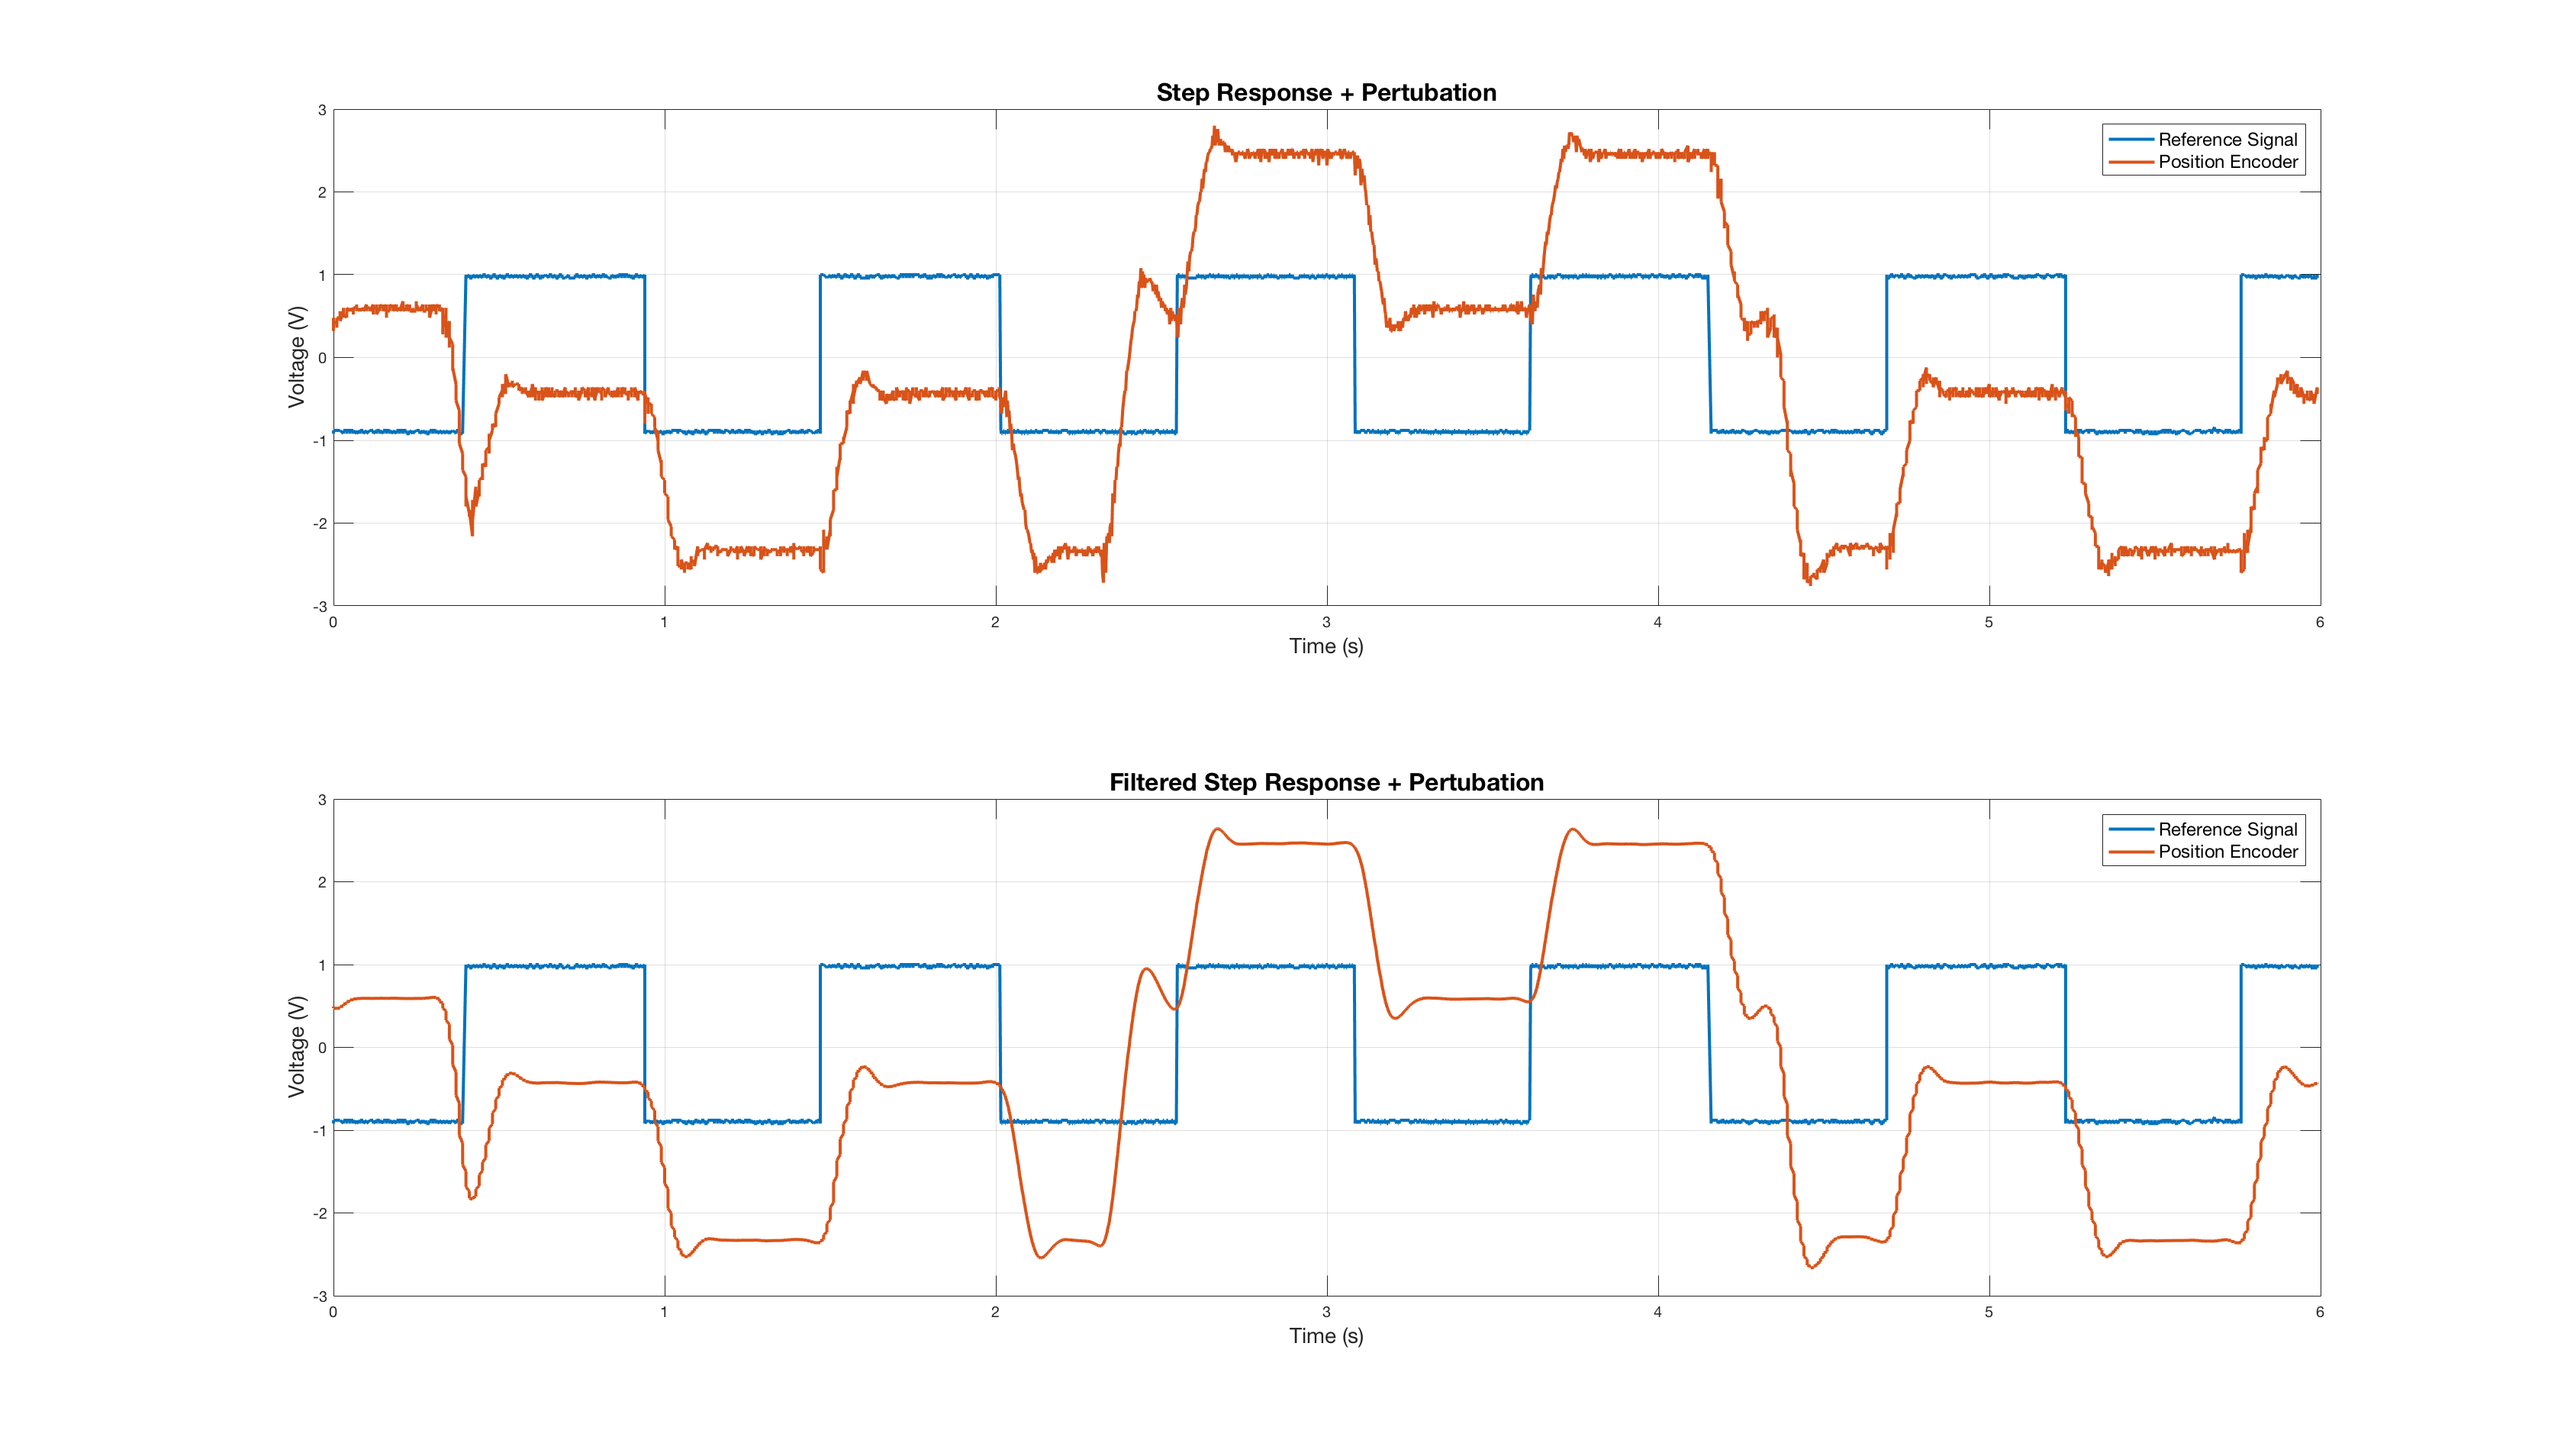
\includegraphics[width=1.1\textheight]{img/results/step_noise.png}
    \caption{Resposta do sistema à entrada degrau unitário com pertubação de $0.25 Hz$ e $2V$ pico a pico. Tanto o sinal de referência, como o sinal de perturbação foram gerados por gerador de sinais. O sinal de posição do carro foi lido da saída PWM do sistema Arduino. Estão representados tanto o sinal original lido no osciloscópio, como um sinal filtrado para remover ruídos de alta frequência.}
    \label{fig::step_noise_response}
\end{sidewaysfigure}
